\makeatletter
\def\input@path{{../}}
\makeatother

\documentclass[/main.tex]{subfiles}

\begin{document}
\graphicspath{{./pics/}{ch3/pics/}}

\textpages
\chapter{Simulating the \MJD}

\section{Simulation Software}
\subsection{\Mage}
\Mage\ (Majorana/Gerda) \cite{mage2011} is a Monte Carlo software package developed jointly by the \MJ\ and \Gerda\ collaborations for the purpose of simulating low-background experiments involving HPGe detectors.
\Mage\ is written primarily in \cpp\ and is based on the \geant\ physics simulation framework\cite{geant2003}.
A \geant\ simulation requires the following inputs:
\begin{itemize}
\item{\textbf{Experiment Geometry:}}
  A discription of the physical dimensions, location, and materials must be provided.
  These should be included for both the detectors and the experimental structure surrounding the detectors.
\item{\textbf{Event Generator:}}
  A generator creates the initial conditions for an event, including the initial particles generated, and the intitial positions and momenta of each initial particle.
  The initial positions will typically be sampled from a particular subset of the full experimental geometry, such as the volume defined by a particular component.
  The initial momenta will be sampled from the allowed phase space of the process, conserving energy and momentum and sampling the angular correlation distribution.
  Many processes will generate multiple events; for example, a \Th{228} decay will generate a set of particles for each decay in the chain, including $\gamma$s generated by nuclear deexcitations.
\item{\textbf{Physics Lists:}}
  The physics lists describe the physical processes to be simulated as the generated particles propagate through the experimental geometry.
  Examples of such processes include Compton scattering of $\gamma$-rays in matter and energy deposition of electrons as they propagate through matter.
  A physics list will describe the probability of a process happening in a given material, any changes to the particle that generated the process, and any new particles produced by the process.
\end{itemize}
\Mage\ contains geometries describing various detector configurations for the \MJD.
\Mage\ also includes event generators that are used to describe \bb from inside the detectors, backgrounds generated by various experimental components from various isotopes, and the line sources used in detector calibration.
Finally, \Mage\ includes the relevant physics lists to the nuclear processes observed by the \MJD.
\Mage\ enables a user to select a geometry and event generator by writing a simple macro and running the \texttt{MaGe} executable on that macro.
All simulations described in this chapter will use the full as-built \MJD\ geometry, which is shown in figure~\ref{fig:mageasbuilt}.
\\
\begin{figure}[h]
  \centering
  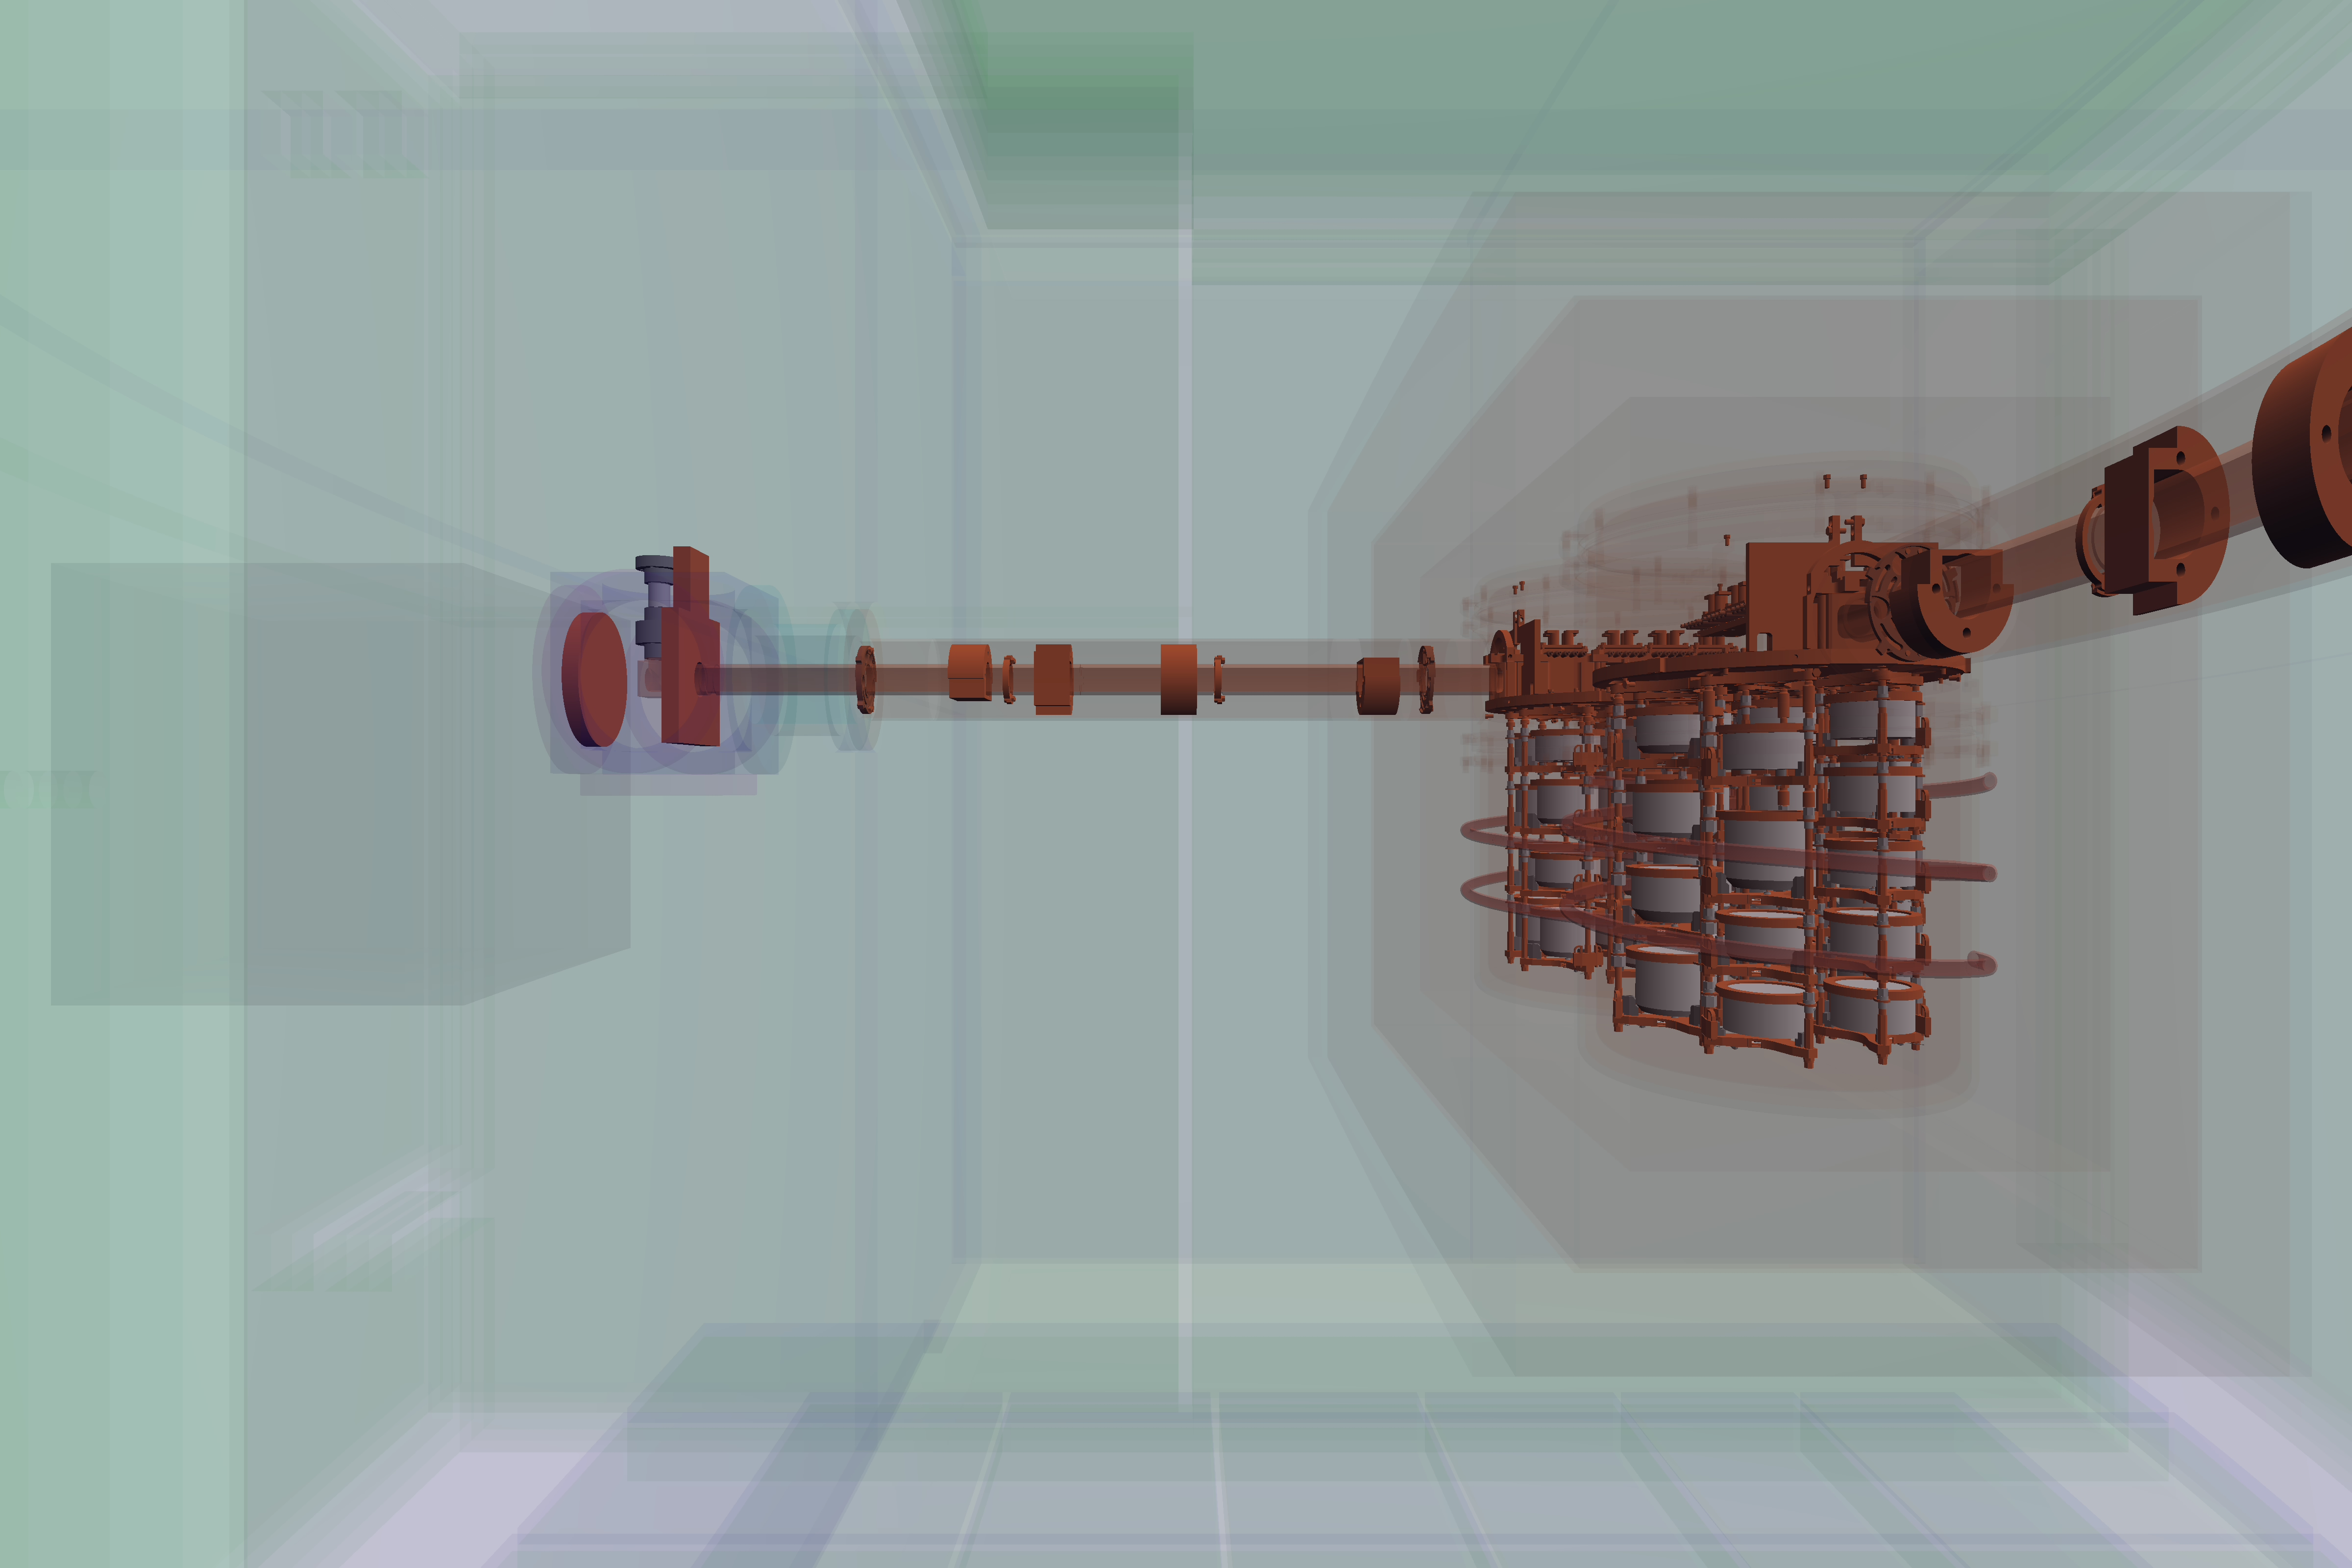
\includegraphics[width=0.8\textwidth]{Geant4Geom.jpeg}
  \caption[The \MJD\ as built simulated geometry]{\label{fig:mageasbuilt}
    The as-built \MJD\ geometry as programmed in \Mage.
  }
\end{figure}

A Monte Carlo run by \geant\ will generate a large number of event primaries.
A Monte Carlo event primary begins with the set of particles created by the input event generator.
Each particle will then be given a particle track, describing the path it takes through the experiment geometry.
If the particle undergoes an interaction with the experiment as described in a physics list, the particle track will end and a Monte Carlo step will occur.
A Monte Carlo step describes the particle before and after an interaction, any additional particles generated in the interaction, and the amount of energy imparted into the matter at the site of the interaction.
For each Monte Carlo event primary, \Mage\ will record an event with the details of each Monte Carlo step that occurs inside of a detector, including the position of the step, the incoming particle, the outgoing particles, the physics process that caused the step, and the amount of energy deposited.
If no interactions occur inside of a detector, no event will not be recorded, but recorded events are enumerated according to the event primaries to ensure that the detection efficiency can be accurately counted.
\\
The simulation events are stored in a \TTree\ containing the following branches:
\begin{itemize}
\item{\texttt{fMCRun}:}
  Contains meta-information about the simulation run, including the run number, number of events, and settings for the run.
\item{\texttt{eventHeader}:}
  Contains meta-information about the event such as the event ID.
\item{\texttt{eventSteps}:}
  Contains data from each event step that deposits energy in a HPGe detector volume, including the location, process and energy deposition.
\item{\texttt{eventPrimaries}:}
  Contains data from the first step in an event, which generated the event.
\end{itemize}

\subsection{Simulation Post-Processing} \label{sec:simpostproc}
Once a \Mage\ simulation is run, the data generated must be post-processed to look like \MJD\ data.
Post-processing is performed by the GAT executable \texttt{process\_MJD\_as\_built\_mage\_results}.
The post-processor requires the input of individual detector characteristics such as energy resolution and dead layer parameters, which are provided via a JSON file.
The relevant steps of the posts-processor will be described in the next few paragraphs.
\\
First, steps within 0.1~mm and 5~ns of each other are grouped into clusters.
A typical cluster will contain the initial physics process that generated the cluster, such as a Compton scatter or $\beta$ decay which generate a high energy electron in the detector, and many electron scatters as the electron comes to rest inside of the detector, generating a cloud of electron-hole pairs.
For each cluster, the total energy and energy-weighted average position of the cluster are computed.
\\
The effect of the detector dead layers are computed for each step individually.
The fraction of total charge collected is modelled as a function of depth beneath the detector surface by the piecewise function
\begin{equation}
  \label{eq:dlmodel}
  A(x) = \begin{cases}
    0 & z < 0 \\
    g(x)=Ae^{Bx} + C & 0 \leq z < t \\
    h(x)=Mx + D & t \leq z < 1 \\
    1 & t \geq 1
  \end{cases}  \qquad
  \text{Constrained to: } \begin{cases}
    g(0)\equiv 0 \\ g(t)\equiv h(t)\equiv f \\ g'(t)\equiv h'(t) \\ h(1)\equiv 1
  \end{cases}
\end{equation}
where $x$ is the depth of the event as a fraction of the dead layer thickness, $t$ is the transition depth, $f$ is the transition fraction, and all other parameters are uniquely determined by $t$ and $f$ \cite{giovenetti2015phd}\cite{buuck2018}.
For each cluster, the uncollected charge is summed and used to compute the deadness fraction for the cluster.
The total measured energy is computed by summing the energy of each cluster, degraded by a factor of its deadness, in a single detector.
The deadness model parameters are measured by performing a fit of a simulated \Th{228} calibration spectrum to calibration data, floating the dead layer parameters for each detector.
The most sensitive parts of the calibration spectrum in this fit are the low energy portion of the spectrum, where events occur in the transition layer and have degraded energy, and in peak heights.
The parameters for this model are provided individually for each detector in a JSON file input to \texttt{process\_MJD\_as\_built\_mage\_results}.
Figure~\ref{fig:calwithdl} shows the best fit of a \Th{228} calibration simulation to data with and without this dead layer model applied.
\begin{figure}
  \centering
  \subfloat[Flat dead layer model]{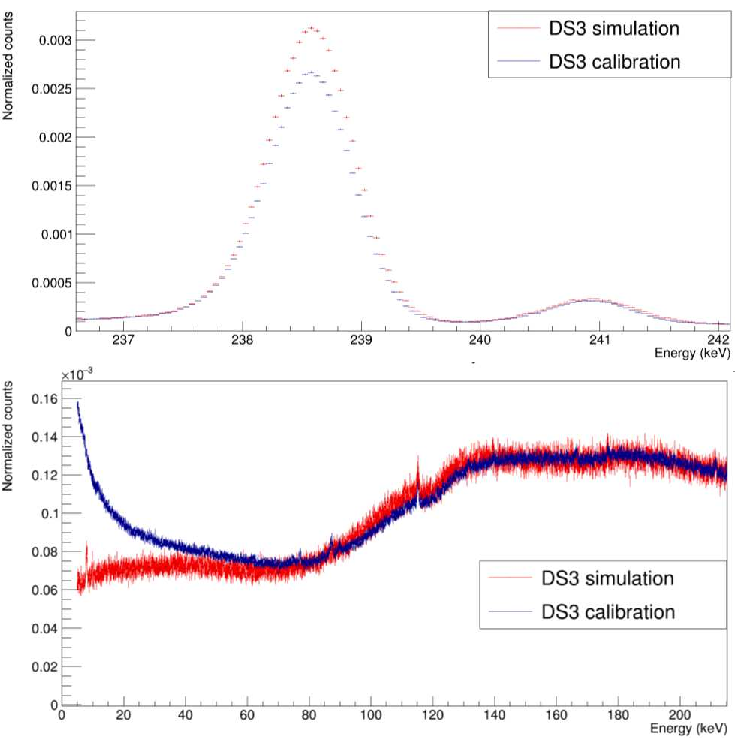
\includegraphics[width=0.5\textwidth]{calspectrum_noDL}}
  \subfloat[Full dead layer model]{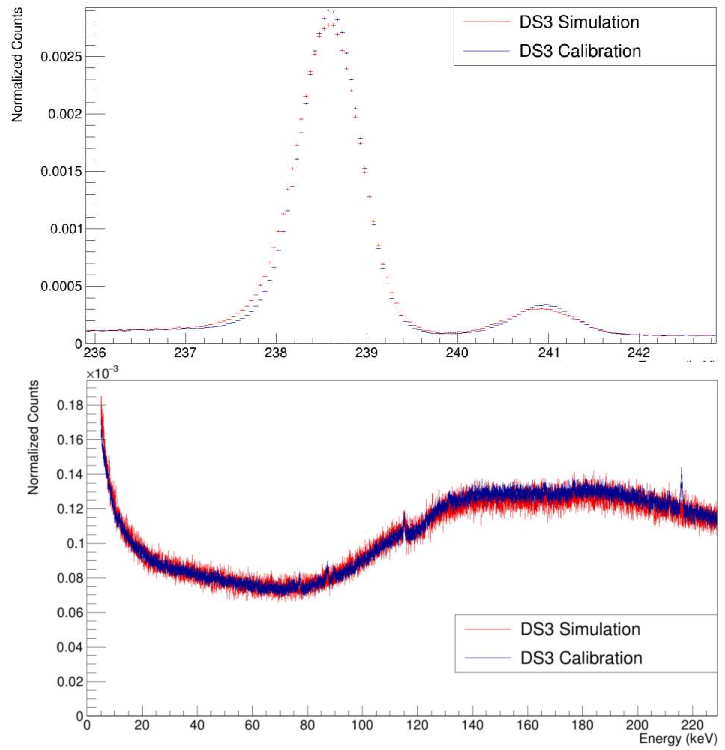
\includegraphics[width=0.5\textwidth]{calspectrum_yesDL}}
  \caption[Comparison of calibration simulation to data with different dead layer models]{\label{fig:calwithdl}
    Comparison of the best fit of a \Th{228} calibration simulation spectrum to calibration data. On the left, a flat, step-like dead layer model is used, and on the right the dead layer model described by equation~\ref{eq:dlmodel} is used. The affect of the dead layer model can be seen the most strongly in the relative peak heights and in the low energy portion of the spectrum. This model fit is used to measure the dead layer thickness and the uncertainty in the thickness.
  }
\end{figure}
\\
Finally, the post-processor smears energies by the response function measured during \Th{228}\ calibration runs.
The post-processor uses the peakshape functions described in appendix~\ref{appendix:peakfitter}.
Only the gaussian and low energy tail parameters are used.
The post-processor samples an energy from the probability distribution described by the peak-shape function centered at the energy calculated for the event.
The peak-shape parameters are provided individually for each detector using the input JSON file.

\subsection{Simulation Skimming} \label{sec:simskim}
Finally, skim files are produced containing parameters of interest from the post-processed files using the software \texttt{es\_skimsims}.
Skim files also mix postprocessed files from multiple sources in ratios corresponding to the various activities of the sources.
\texttt{es\_skimsims} accepts as input a json file listing the simulated sources, the desired activity of each source, and the number of available event primaries.
From this, it calculates the number of primaries to accept from each source by maximizing the total number of events used while mainting the correct ratio according to the activities.
Once this is done, it goes through each source sequentially and saves parameters of interest, including energy and detector position to a \texttt{TTree}.
As will be discussed in future chapters, single detector events are of little interest to this analysis, so only \msmd\ events are recorded in order to maintain a small file size.
Multiplicity 1 events are recorded separately to a histogram according only to energy.
The skimming process also accounts for which sets of detectors are enabled.
Another input of \texttt{es\_skimsims} is a json file containing a list of detector configurations, containing a bitmask describing which detectors are and are not enabled.
The detector configurations will be discussed further in section~\ref{sec:sds}.
When the skimmer encounters a disabled detector in an event, it ignores that detector, and does not count it towards the event multiplicity.
\\
 
Each detector spends some portion of operating time dead, due to the finite rate at which the digitizers can retrigger, which can cause up to $\sim1$\% of HPGe hits to fail to read.
This effect is assumed to be random and uncorrelated between detectors.
The dead time of each detector is measured by counting the number of pulser events in each detector for each run.
Because the pulses occur at a fixed rate, we can predict the number of pulser events that should occur in any given run; the fraction of pulser events missed is assumed to represent the dead time.
The json detector configuration file contains the dead time fraction and the statistical uncertainty on that fraction for each active detector.
For each simulated detector hit, the data skimmer randomly throws out hits according to the the probability represented by the dead fraction, treating that detector as inactive for that event.

\section{Simulation of Excited State Decays} \label{sec:essims}
Simulations of the \Ge{76} decay to excited states of \Se{76} are used to evaluate the detection efficiency of the analysis presented in this document.
Two different event generators are used to generate \Ge{76} \bb-decay\ within \Mage.
The first generator uses calculations of the phase space factors from J.~Kotila and F.~Iachello\cite{Kotila2012}.
It is implemented in the mage class \texttt{MGGeneratorDoubleBeta} using data tables with the distribution of both electron energies and anglular correlations.
These data tables are provided for the \tnbb\ and \znbb\ decays to the ground state of \Se{76}, but not for the decays to any excited state of \Se{76}.
This calculation is an improvement over other phase space calculations thanks to an exact evalutation of the Dirac wave functions of the electrons involving a finite nuclear size and electron screening.
\\
A second event generator packaged with \Mage\ is \texttt{decay0}\cite{Ponkratenko2000}, a fortran program that generates a wide variety of $\beta\beta$- and $\beta$-decays.
\texttt{decay0} is capable of generating \tnbb\ and \znbb\ for \Ge{76} to \Se{76} \SP{0}{+}{} and \SP{2}{+}{} excited states using a variety of physics mechanisms.
For the excited state decays, the deexcitation $\gamma$s and conversion electrons are also generated.
Several modifications were made to \texttt{decay0} for this analysis.
First, the precision of the excited state deexcitation energies was increased from 1~keV to 0.001~keV (The $\gamma$ energies changed from 559 to 559.101~keV, from 563 to 563.178~keV, from 657 to 657.041~keV, and from 1216 to 1216.104~keV).
Second, angular correlations were added for the \SP{2}{+}{2}-\SP{2}{+}{1}-\SP{0}{+}{g.s.} deexcitation $\gamma$ cascade which involves a 657~keV $\gamma$ with multipolarity E2+M1 and mixing ratio of $+5.2$ followed by a 559~keV $\gamma$ with multipolarity E2\cite{SINGH1995}.
The angular distribution between the $\gamma$s is
\begin{equation}
  P(\theta)\propto 1-0.372\cdot\cos^2(\theta)+0.0439\cdot\cos^4(\theta)\cite{Evans1955}
\end{equation}
The angular correlation for the \SP{0}{+}{1}-\SP{2}{+}{1}-\SP{0}{+}{g.s.} deexcitation was previously included in \texttt{decay0}, and is represented by the angular distribution
\begin{equation}
  P(\theta)\propto 1-3\cdot\cos^2(\theta)+4\cdot\cos^4(\theta)
\end{equation}
Running \texttt{decay0} produces data files with the initial momenta of the generated particles.
The \Mage\ class \texttt{MGGeneratorDecay0} reads these datafiles and generates initial positions for these events.
\\
\begin{figure}[h]
  \centering
  \includegraphics[width=.9\linewidth]{ESsim}
  \caption[Simulation of multiplicty 2 events from \tnbb\ to \SP{0}{+}{1}]{\label{fig:2dessim}
    Multiplicity 2 energy spectrum produced by a decay0 simulation of \tnbb\ of \Ge{76} to the \SP{0}{+}{1} state of \Se{76}.
  }
\end{figure}
Simulations were run for \Ge{76} \tnbb and \znbb to the \Se{76} \SP{0}{+}{1}, \SP{2}{+}{1} and \SP{2}{+}{2} excited states using the \texttt{decay0} generator.
For each decay mode, 5000000 event primaries were generated in the bulk of the enriched detectors and 500000 primaries were generated in the bulk of the natural detectors.
These events were skimmed with the relative activities set equal to the total isotopic mass in each set of detectors: 26.2538~kg in enriched detectors, and 1.1232~kg in natural detectors.
These simulations were additionally post-processed with the dead layer thickness set to 0, and skim files were produced both with and without a dead layer, and with and without dead times.
Figure~\ref{fig:2dessim} shows an energy spectrum of multiplicity~2 events produced by the simulation of the \Ge{76} decay to the \SP{0}{+}{1} excited state of \Se{76}.
\\
\subsection{Comparing \texttt{decay0} to the Kotila and Iachello generator}
\begin{figure}
  \centering
  \subfloat[\texttt{decay0} \tnbb\ to g.s.]{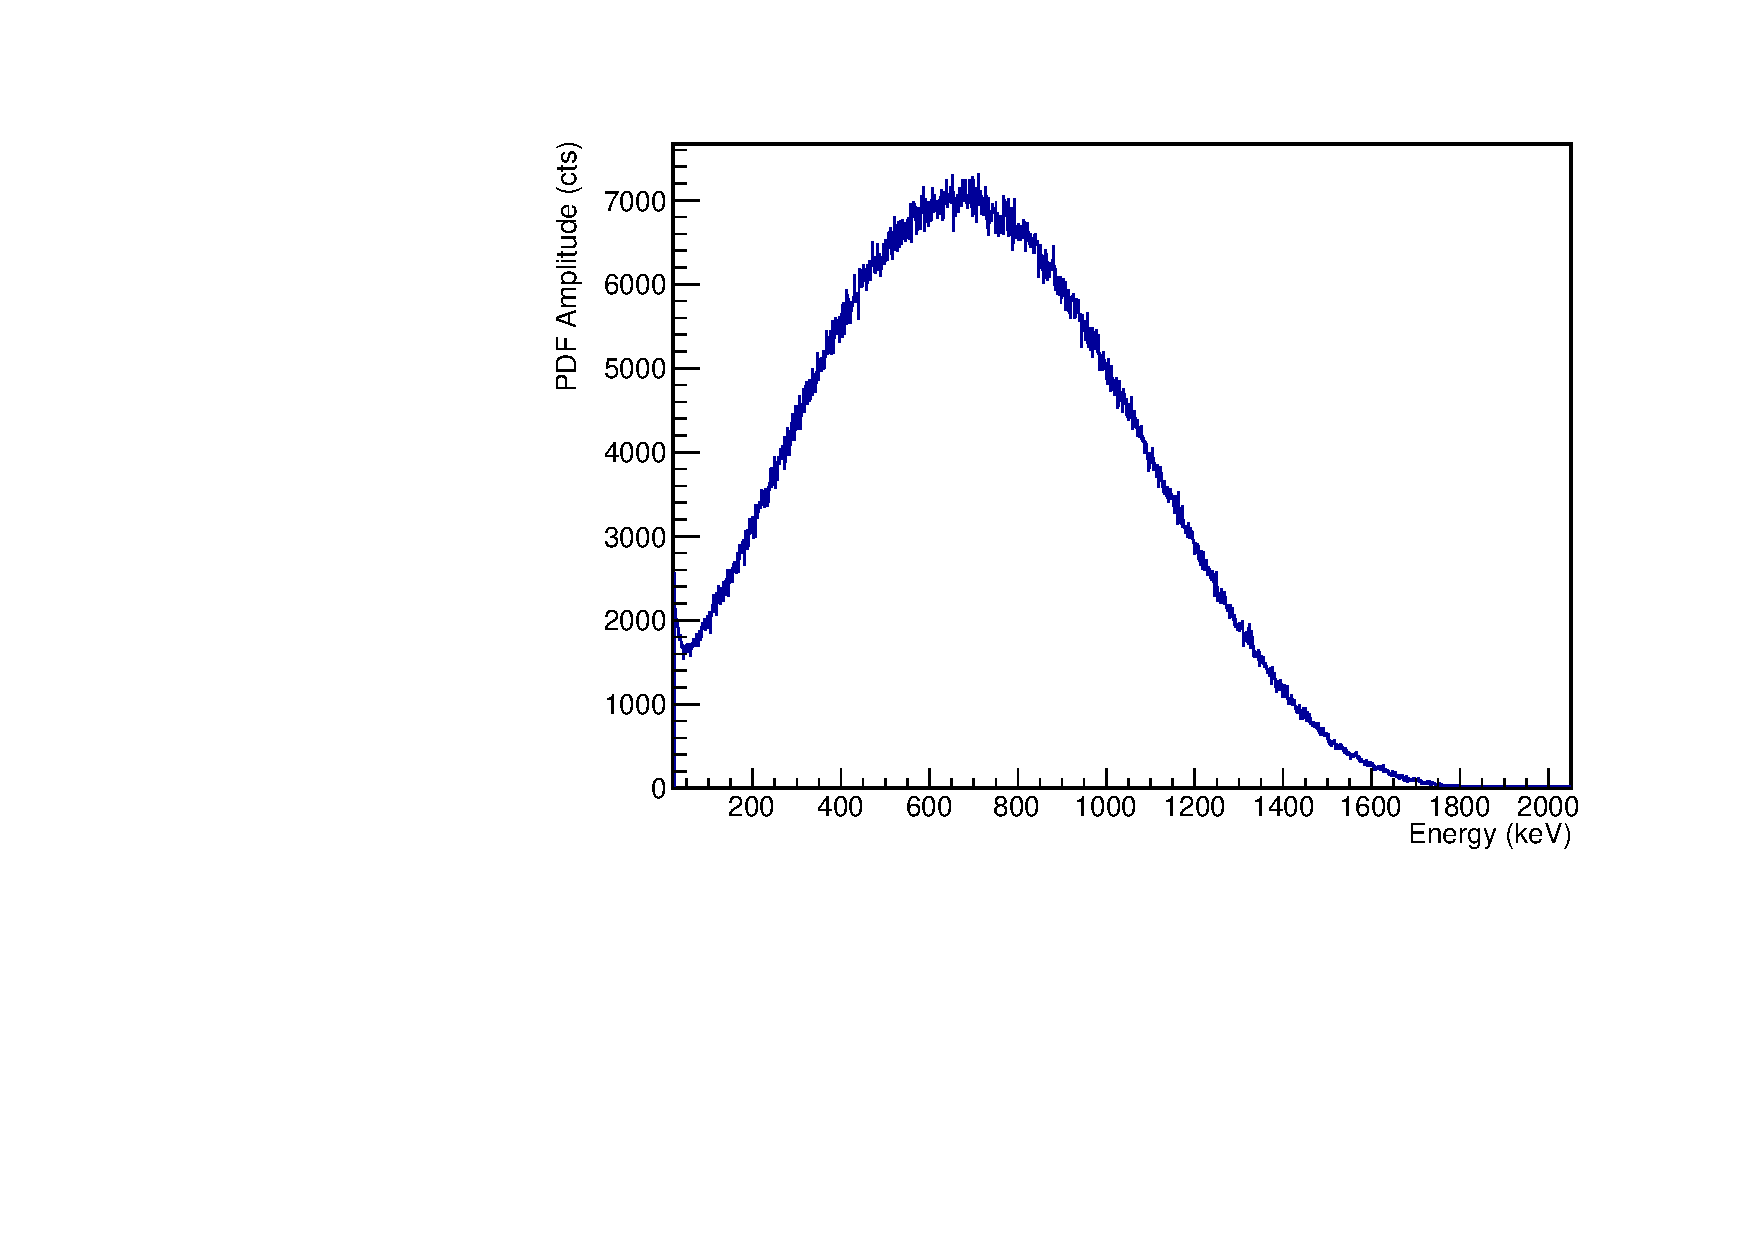
\includegraphics[width=0.5\linewidth]{decay0gsspectrum}}
  \subfloat[CDF difference]{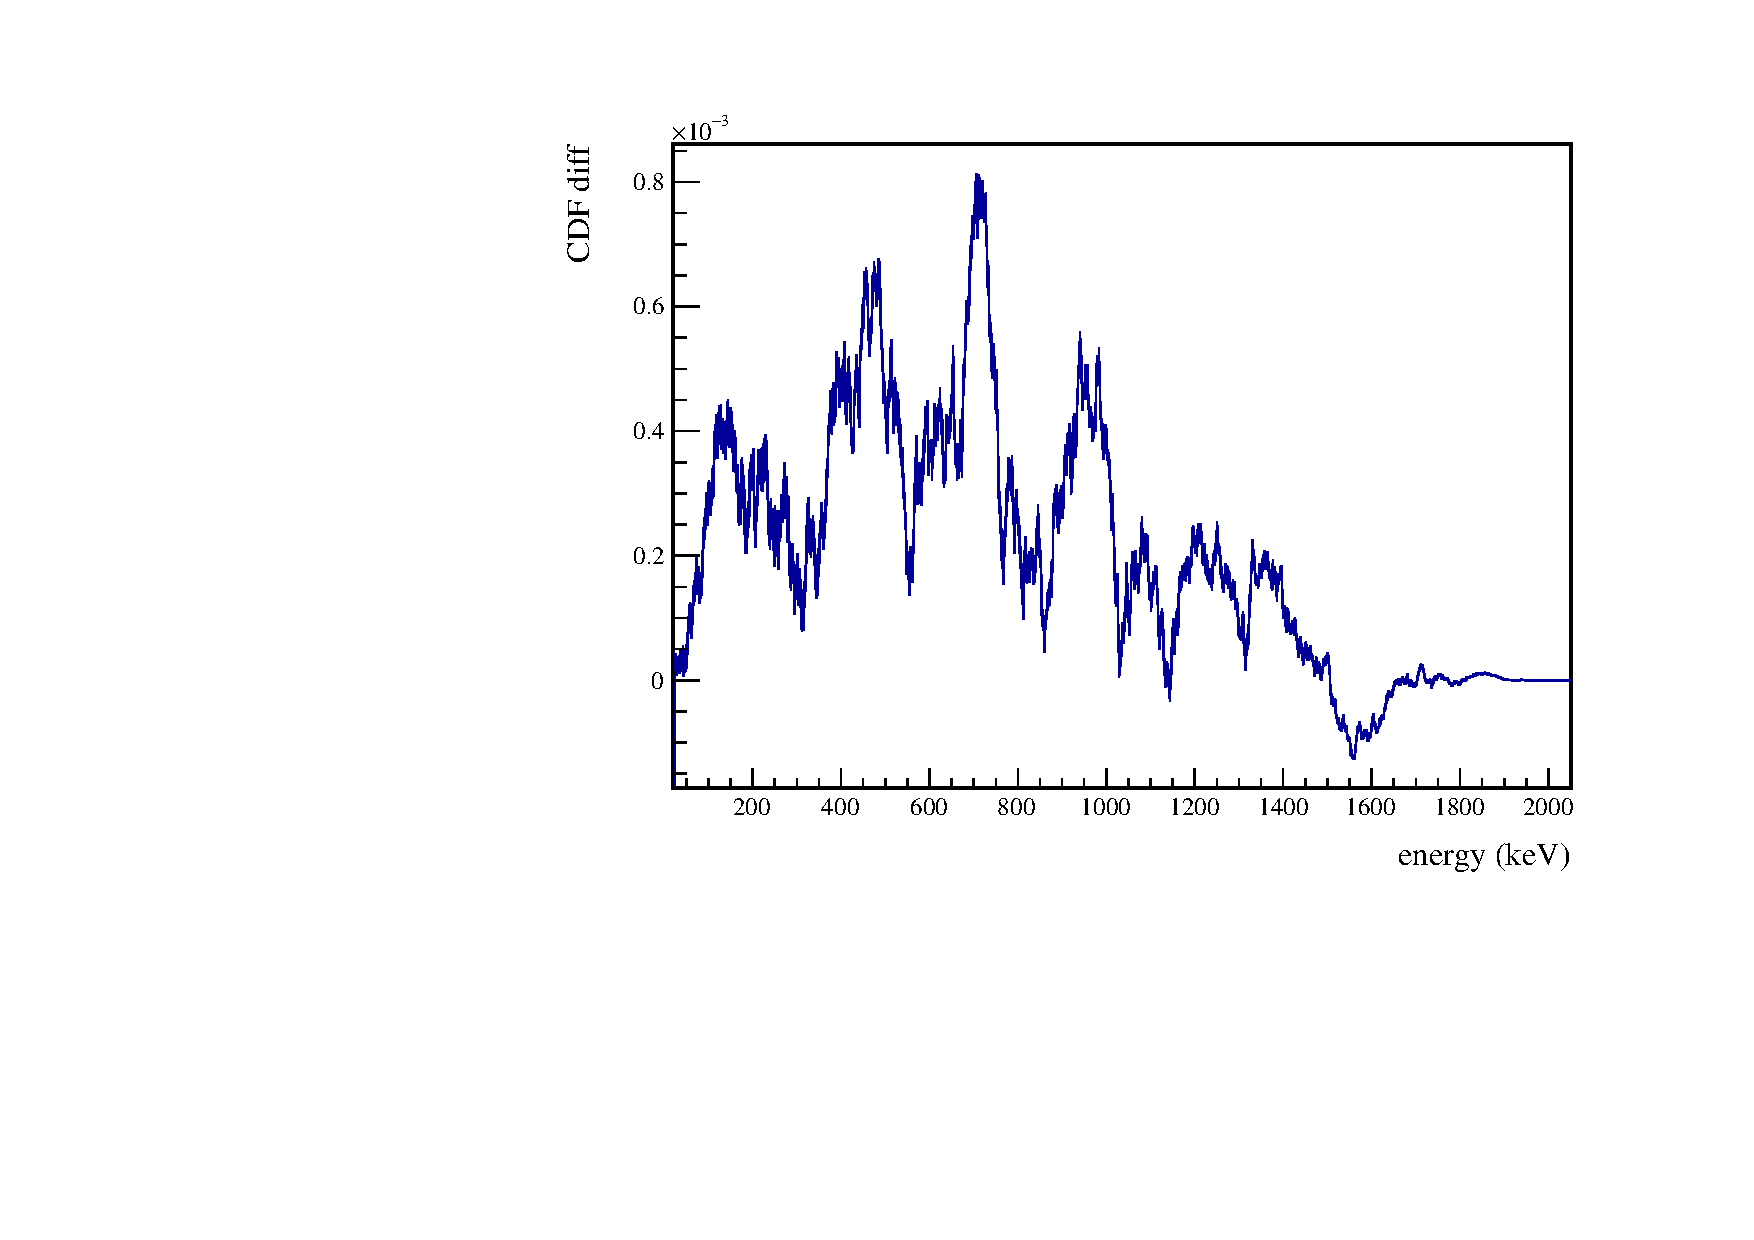
\includegraphics[width=0.5\linewidth]{decay0KS}}
  \caption[KS test comparing \texttt{decay0} to Kotila and Iachello \tnbb to g.s. spectra]{\label{fig:kstest}
    A KS test is performed comparing the \texttt{decay0} \tnbb to the ground state energy spectrum to that of Kotila and Iachello. The \texttt{decay0} spectrum is shown, along with the difference between the CDF of each spectrum.
  }
\end{figure}
The Kotila and Iachello generator performs a more calculation of phase space than \texttt{decay0} and is used for the \MJD 's measurement of \tnbb\ and \znbb\ to the ground state.
Because Kotila and Iachello present only the phase space integral for the excited state decays, and do not include the energy and angular distributions, \texttt{decay0} is used for this analysis.
To evaluate the accuracy of \texttt{decay0}, we can compare the spectrum of the \tnbb\ to the ground state it generates to that of Kotila and Iachello; this comparison will reflect the error with respect to the true value if we assume that the error on the latter spectrum is much smaller than that of \texttt{decay0}.
This comparison is performed using a Kolmogorov-Smirnov (KS) test.
The KS test statistic is the maximum difference between the CDF of each normalized energy spectrum.
As we will see in chapter~\ref{chap:ch4}, this test is useful in evaluating the uncertainties in the measurement presented in this thesis.
The CDF difference is shown in figure~\ref{fig:kstest}, with a KS statistic of 0.00081.
While this error is statistically significant at a level of 97\%, we will see that the systematic error generated is subdominant.

\section{Background Model Simulation}
A simulation of the background spectrum measured by the \MJD\ will be used to optimize the search for \bbes.
\Mage\ simulations of a variety of decay chains, including \Th{232}, \iso{238}{U}, \iso{40}{K}, \Co{60}, \iso{222}{Rn} and \Ge{68}, have been run using event generators internal to \geant.
Geometries of large number of component groups have been defined encompassing one or more physical component of the experiment.
Decays can be generated in either the bulk of a component group, or on the surface.
The activity of each isotope from each component group is determined by fitting a linear combination of the simulated energy spectra to the measured background spectrum.
An incomplete version of this fit is used for this thesis, producing the spectra in figures~\ref{fig:bgsim1D} and~\ref{fig:bgsim2D}.
\Ge{68} decays with a half-life of 271~days, so its activity is scaled to represent the activity of each major dataset.
\iso{210}{Pb} in the lead shield is simulated using a special generator that samples bremstrahlung x-rays emitted from the surface of a thick lead shield \cite{VOJTYLA1996}.
\\
\begin{figure}
  \centering
  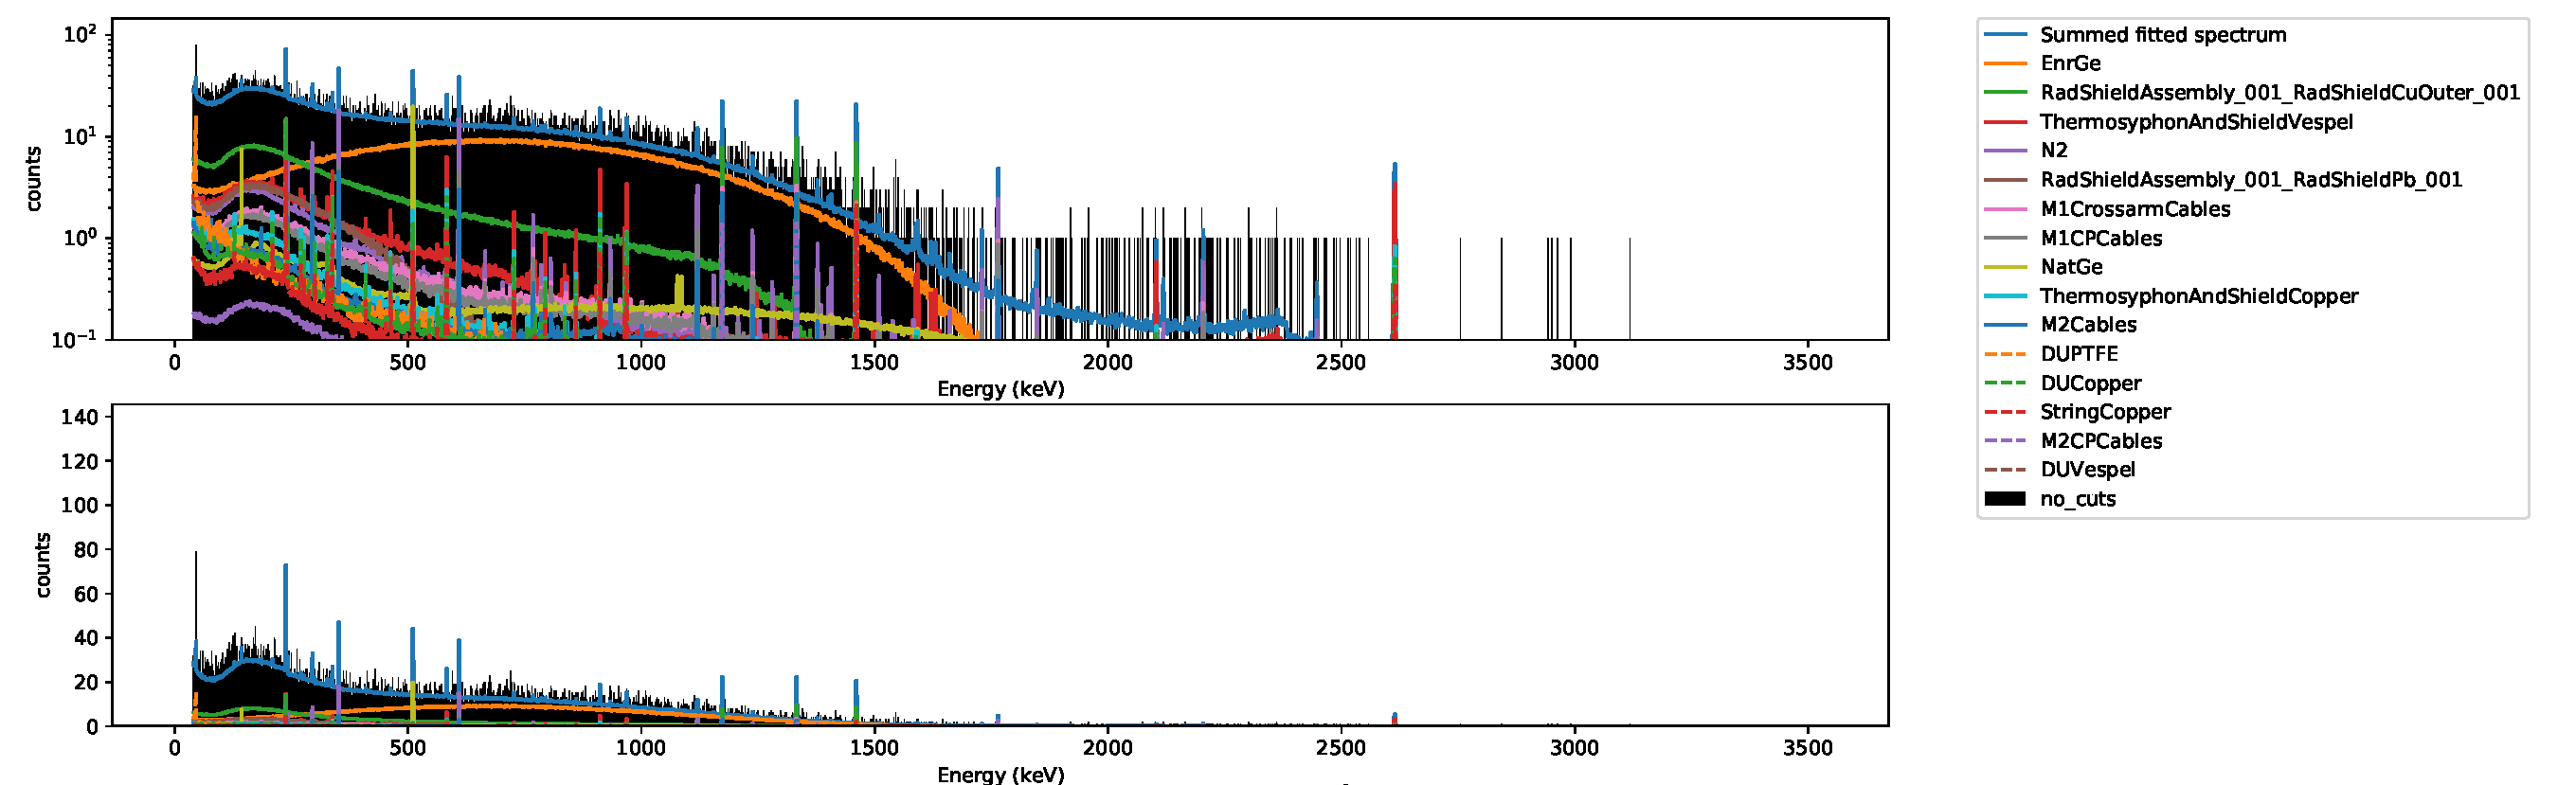
\includegraphics[width=1\linewidth]{BGsim1D}
  \caption[Simulation of multiplicty 1 events from the background model]{\label{fig:bgsim1D}
    Energy spectrum of multiplicity 1 events produced from a simulation of the background model, with most common source components labelled.
  }
\end{figure}

\begin{figure}
  \centering
  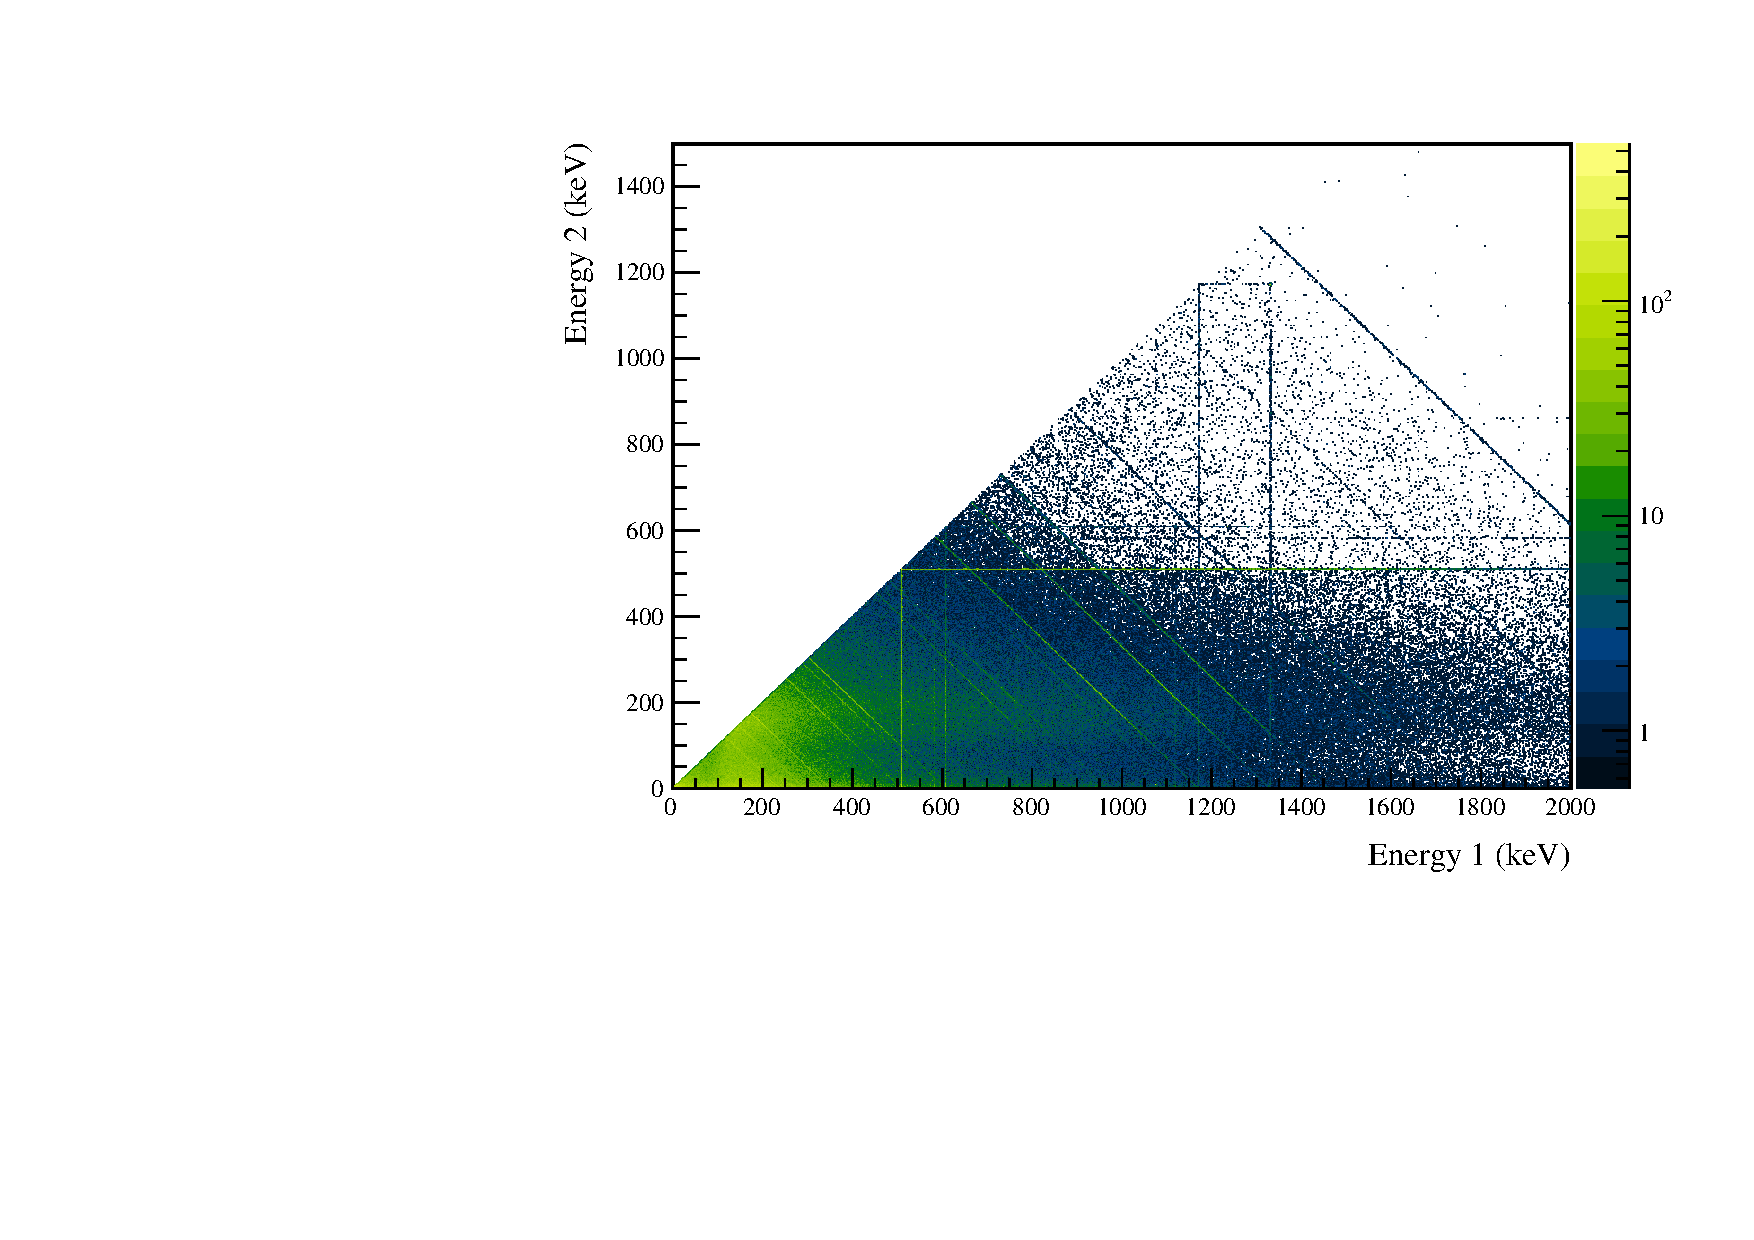
\includegraphics[width=.9\linewidth]{BGsim2D}
  \caption[Simulation of multiplicty 2 events from the background model]{ \label{fig:bgsim2D}
    Multiplicity 2 energy spectrum produced by a simulation of a preliminary version of the \MJD\ background model.
  }
\end{figure}
The background model used for this analysis is known to be inaccurate.
Since it is only used for optimizing the search for \bbes\ and is not important for the detection efficiency calculation, this does not affect the accuracy of the result presented.
For future versions of this analysis, a complete and more accurate background model will be used, which will result in small improvements to the optimization.

\section{Calibration Source Simulation}
Calibration of the \MJD\ is performed for each module using using a line source that is injected by motor into a spiral track that winds around the module.
Both \Th{228} and \Co{56} line sources are used.
Simulations of each of these calibration sources are performed using the \geant\ generators for these isotopes, and a spiral position sampler written in \Mage.
These simulations are used to test various aspects of the \Mage\ simulations and to calibrate several observables.
For example, the dead layer thickness measurement described in section~\ref{sec:simpostproc} relies on the \Th{228} source simulation, and the detection efficiency test described in section~\ref{sec:Co56} uses the \Co{56} source simulation.
The simulated spectra for the \Co{56} source can be seen in figures~\ref{fig:56Co1D} and~\ref{fig:56Co2D}
\begin{figure}
  \centering
  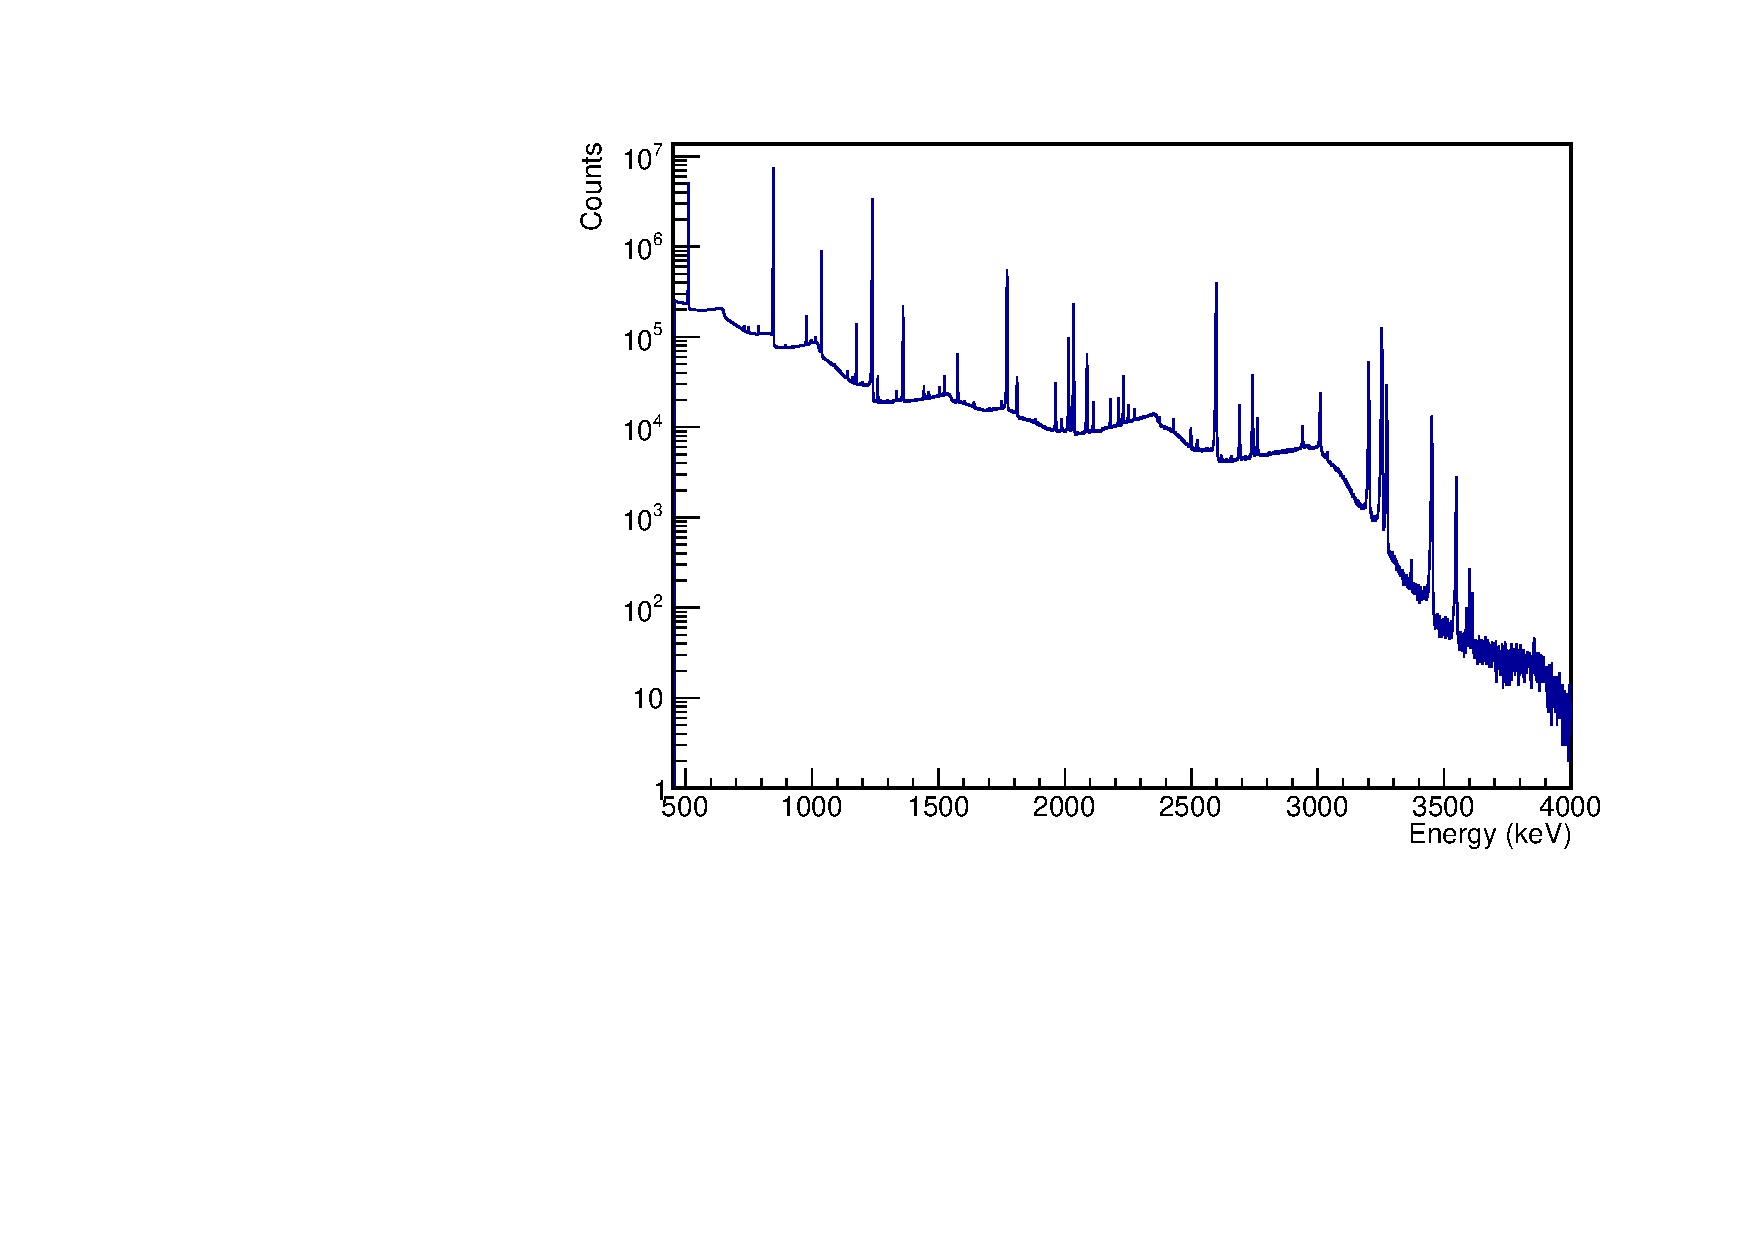
\includegraphics[width=.8\linewidth]{Co56Sim1D}
  \caption[Simulation of multiplicty 1 events from \Co{56} line source]{ \label{fig:56Co1D}
    Energy spectrum of multiplicity 1 events produced from a simulation of the \Co{56} line source inserted into the module~1 calibration track.
  }
\end{figure}

\begin{figure}
  \centering
  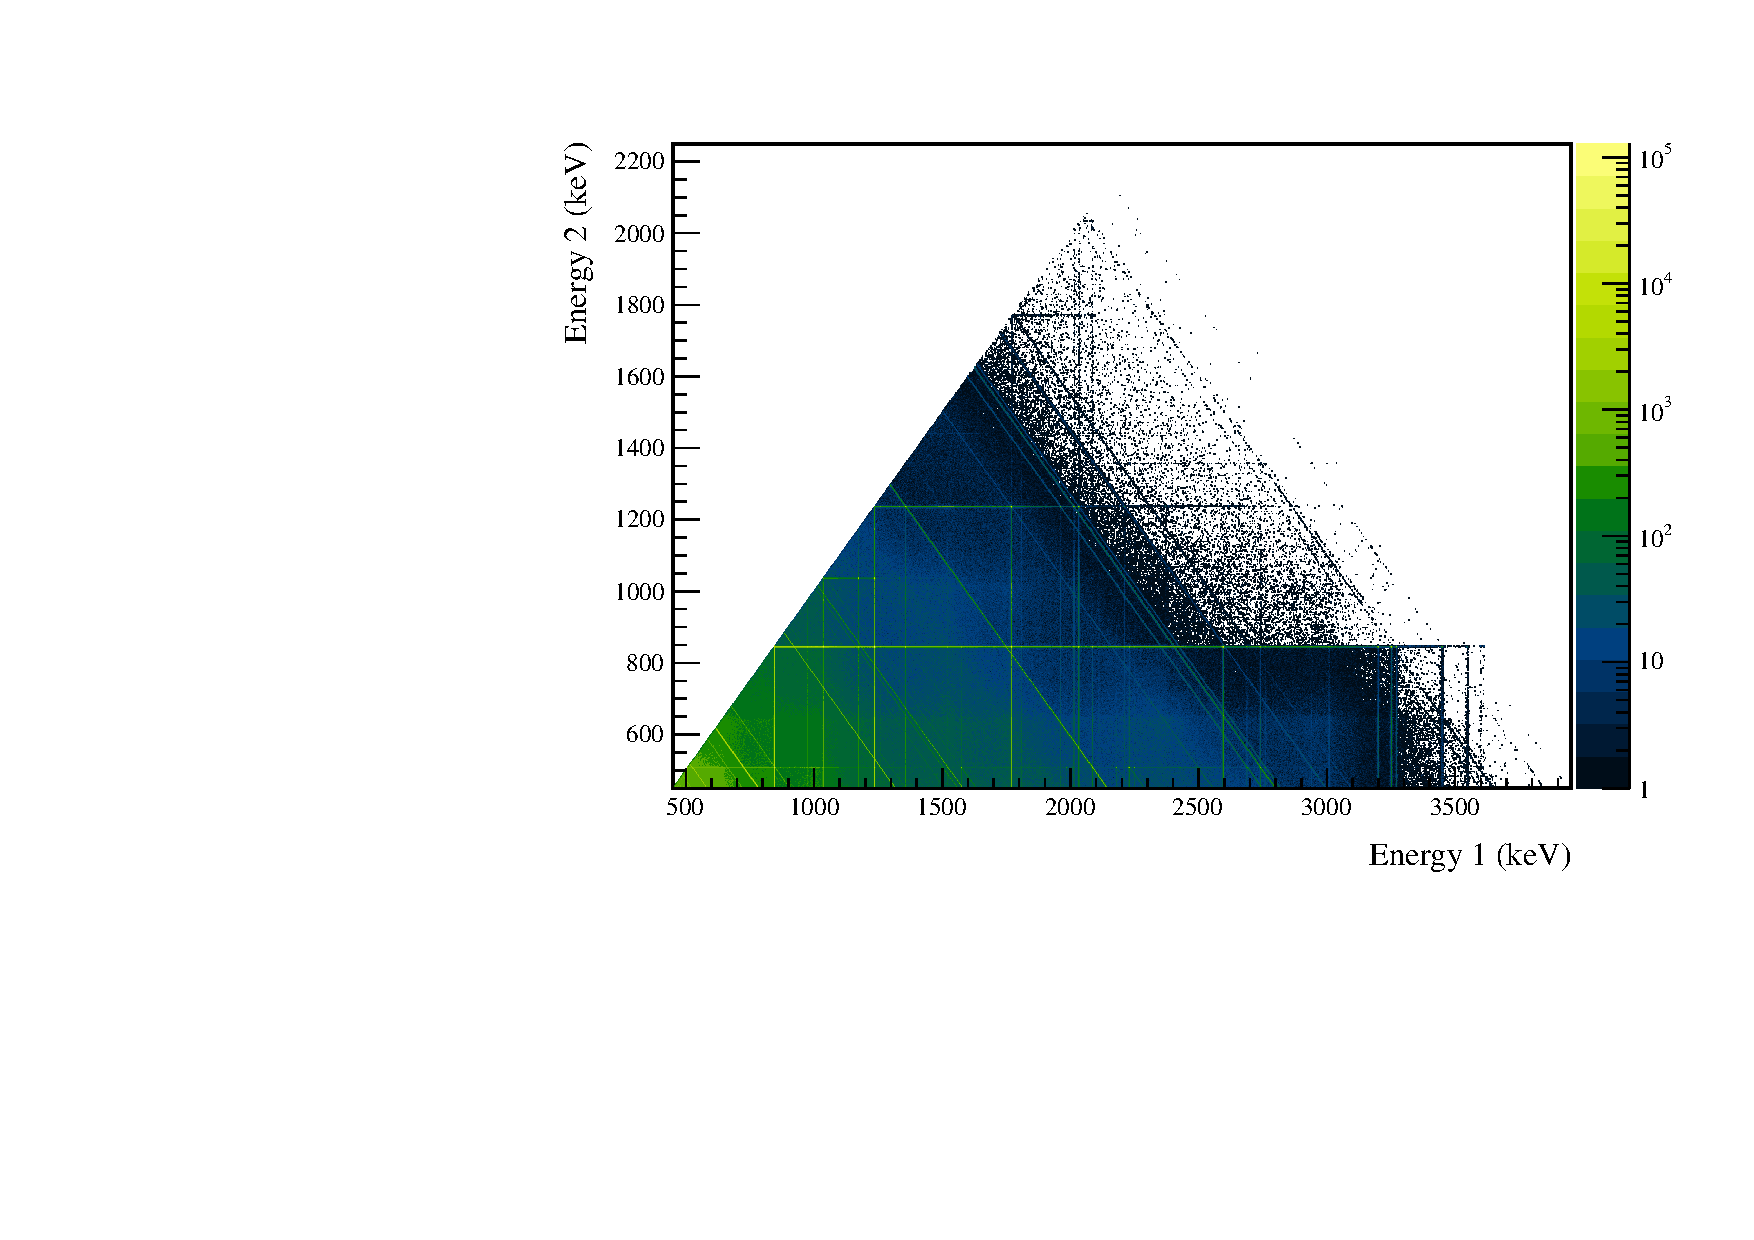
\includegraphics[width=.8\linewidth]{Co56Sim2D}
  \caption[Simulation of multiplicty 2 events from \Co{56} line source]{ \label{fig:56Co1D}
    Multiplicity 2 energy spectrum produced by a simulation of the \Co{56} line source inserted into the module~1 calibration track.
  }
\end{figure}


\end{document}
